\chapter{La composante embarquée}
\section*{Introduction}
Rappelons que nous visons embarquer notre solution intélligente sur un drone. Ce drone est sensé de survoler le terretoire du l'agriculteur et de donner une estimation sur la quantité de sa production. 
Le premier défis qui s'impose 
\section{Anatomie du drone}
\subsection{Liste des composants}
\subsection{Flux d'information}
\subsection{Discussion}
\section{Intégration de la composante intélligente}
\subsection{Préparations}
\subsection{Problèmes d'intégration}
\subsection{Interfeçage}



Les systèmes embarqués font partie intégrante de nos vies. Les personnes ont maintenant un système embarqué, à la maison, dans leur véhicule ou directement sur eux même .On compte actuellement plus d'un milliards, chacun avec ses propres caractéristiques, couvrant tous les secteurs,
que ce soit l'aviation, les appareils, les téléphones et même les voitures. L'amélioration de la qualité
des produits et l'ajout continu de nouvelles fonctions sont directement attribuables à l'intégration des
systèmes embarqués qui, dans un contexte de développement économique, augmentent la compéti-
tivité des entreprises manufacturières tout en créant de la valeur ajoutée. En effet, les domaines de
Recherche et de Développement centrés sur l'IA explorent cette nouvelle voie. Il est particulièrement
intéressant de trouver des moyens de réduire la taille des algorithmes afin qu'ils puissent fonctionner
sur des puces de faible puissance qui sont elles-mêmes installées dans des voitures, des machines in-
dustrielles ou des appareils électroménagers. Cette forme d'IA intégrée existe déjà : elle identifie les
types d'activité physique via des capteurs de smart-phone, l'engagement vocal sur les appareils grand
public, la surveillance des appareils IoT industriels et la distinction des personnes dans les caméras.
Hormis de nouveaux usages, ces puces réduites consomment très peu. Alors que l'IA est considérée
comme une activité extrêmement énergivore, elle ouvre de nouveaux horizons pour continuer à progresser dans le domaine sans impacter les factures énergétiques et l'empreinte carbone des industriels.
\newline
Dans le cadre du déploiement du système de détection des plantes dans des champs à l'aide de drones,
nous avons choisi d'utiliser une carte nommée "Raspberry Pi " et nous avons bien étudié ce choix.
\newline
dans ce chapitre nous allons justifier le choix du Raspberry Pi en expliquant le rapport entre Raspberry Pi et l'IA et introduire la partie logicielle.
\section{Pourquoi  Raspberry Pi ? }
\subsection{Présentation de  Raspberry Pi:}
La Raspberry Pi est aussi connu sous le nom SBC(Single-Board Computer) ou ordinateur à carte unique . C'est un nana-ordinateur à la taille d'une carte de crédit possède toutes les fonctionnalités d'un ordinateur réel avec un processeur ARM multicoeurs qui offre des  performances bien supérieure à ces prédécesseurs , une mémoire plus  rapide, un stockage , un pilote graphique, une connectivité complète : Bluetooth,  Wi-Fi, ports USB,  ports HDMI, Broches GPIO,connecteur CSI (pour caméra) et parfois port Ethernet et carte son...   .\\
\vspace{10pt}
\begin{figure}[H]
        \centering 
        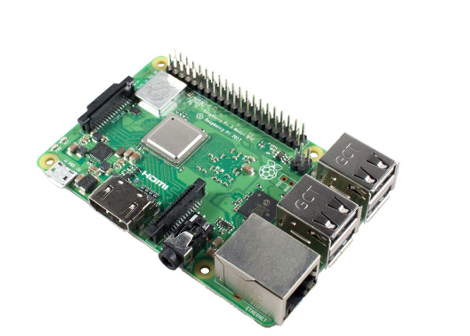
\includegraphics{figures/chap3/raspberry.PNG}
         \caption{raspberry pi SBC}
\end{figure}        
\vspace{10pt}
Puisqu'il y a tous les composants nécessaires à bord, ce Pc miniature peut facilement être connectés à Internet en utilisant le Wi-Fi ou Ethernet  et servir d'interface à de nombreux composants électroniques des LED, des boutons, des capteurs, des moteurs, etc. 
Aussi,on peut  ajouter du matériel externe tel qu'une caméra, un GPS, des panneaux RVB, clavier ,souris,moniteur... .
Comme elle dispose des ports USB,le raspberry peut lire des données depuis un USB ou un disque dur externe.\\
\newline
Les nouveaux modèles de Raspberry Pi ne possède pas de stockage, mais des puces SD  peuvent être utilisées pour stocker les données . Alors, on a la possibilités de transférer les données de notre PC ou ordinateur portable local vers la carte SD et le réciproque.\\
\vspace{10pt}\newline
Un RPi est un ordinateur indépendant et plus ou moins complet , généralement  d'un système d'exploitation Linux basé sur Debian, fourni avec un interpréteur de langage de programmation python. 
c'est pourquoi, elle est multi-plateforme ,le raspberry supporte plusieurs langages de programmation   pour développer des applications comme Python qui existe par défaut, Scratch, Ruby, C, C++, javaScript .\\
Pour cette raison ,le RPi  peut utiliser Python IDLE, Eclipse IDE ou tout autre IDE pris en charge par Linux. on peut également programmer en utilisant le terminal lui-même avec n'importe quel éditeur de texte comme Vim, nano.\\
\vspace{10pt}\newline
 outre à tous ces caractéristiques,  ce nano-ordinateur peut effectuer des processus multitâches . Par exemple,Naviguez avec le navigateur Web sur Internet tandis qu'en arrière-plan, les valeurs des capteurs sont stockées dans une base de données SQL et une sauvegarde est effectuée.\\
 \begin{figure}[H]
        \centering 
        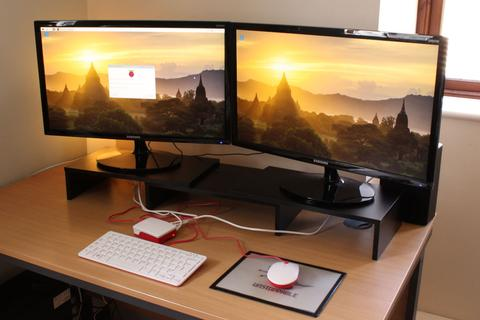
\includegraphics{figures/chap3/Execution-de-deux-moniteurs-avec-un-Raspberry-Pi.jpg}
         \caption{installer deux écrans sur raspberry pi}
\end{figure} 
 \clearpage
 \subsection{raspberry pi 4 vs Arduino vs Esps:}
 Le tableau ci-dessous montre la différence entre le Raspberry Pi 4 et les autres cartes électroniques qu'ils sont souvent considérés comme des solutions concurrentes . La comparaison d'un Raspberry Pi et des microcontrôleurs  est difficile car les systèmes diffères.\\ 

 \begin{table}[H]
    \centering
    \begin{tabularx}{0.9\textwidth} { 
        | >{\centering\arraybackslash}X
        | >{\centering\arraybackslash}X 
        | >{\centering\arraybackslash}X 
        | >{\centering\arraybackslash}X
        | >{\centering\arraybackslash}X |}
        \hline
        & ESP32 & ESP8266 & Arduino UNO & Raspberry pi4\\
        \hline
        Core & Dual code& Single core & Single core &quad-core \\
        \hline
        Architecture & 32 bit LX6 with
        600 DMIPS & 32 bit LX106& 8 bit RISC &64-bit ARM Cortex-A72 \\
        \hline
        Ram & 520Kb  &  128KB  & 264KB   & 1GB/2GB/8GB  \\
        \hline
        Fréquence & 160 Mhz  & 80 Mhz & 16 Mhz & 1.5 GHz \\
        \hline
        Ports Digitaux & 36 & 17 & 14 & 40\\
        \hline
        Ports analogiques & 18 & 1 & 6 & 
        \begin{center}
            \begin{itemize}
                \item 
            \end{itemize}
        \end{center}\\
        \hline
        Bluetooth  Intégré &
        \begin{center}
        \begin{itemize}
            \item 
            \end{itemize}
        \end{center}
            &\begin{center}
        \begin{itemize}
            \item 
            \end{itemize}
        \end{center} & 
        \begin{center}
        \begin{itemize}
            \item 
            \end{itemize}
        \end{center} &
        \begin{center}
        \begin{itemize}
            \item
            \end{itemize}
        \end{center}\\
        \hline
        WiFi Intégré & 
        \begin{center}
        \begin{itemize}
            \item 
            \end{itemize}
        \end{center}
        &
        \begin{center}
        \begin{itemize}
            \item 
            \end{itemize}
        \end{center}
        &
        \begin{center}
        \begin{itemize}
            \item 
            \end{itemize}
        \end{center}
        &
        \begin{center}
        \begin{itemize}
            \item 
            \end{itemize}
        \end{center}\\
        \hline
        Alimentation USB & 
        \begin{center}
        \begin{itemize}
            \item 
            \end{itemize}
        \end{center}
        &
        \begin{center}
        \begin{itemize}
            \item 
            \end{itemize}
        \end{center}
        &
        \begin{center}
        \begin{itemize}
            \item 
            \end{itemize}
        \end{center}
        &
        \begin{center}
        \begin{itemize}
            \item 
            \end{itemize}
        \end{center}\\
        \hline
        langage de programmation &  Arduino IDE
        C/C++
        Micro Python & Arduino IDE
        C/C++
        Micro Python
        Javascript& Arduino IDE
        C/C++  python  & Perl, Ruby, Python, Java, Lua ,javascript \\
        \hline
        OS & \begin{center}
        \begin{itemize}
            \item 
            \end{itemize}
        \end{center} & 
        \begin{center}
        \begin{itemize}
            \item 
            \end{itemize}
        \end{center}   &  
        \begin{center}
        \begin{itemize}
            \item 
            \end{itemize}
        \end{center} &  distribution Linux basée sur Debian    \\
        \hline
        consommation énergie & 1.08mw & 1.0mw & 175mw & 700mw \\
        \hline
    \end{tabularx}
 \end{table}
\vspace{10pt}
\textbf{Comparaison du système d'exploitation de Raspberry Pi contre Arduino et les NodeMCUs:}\\
\vspace{10pt}
\newline
La Raspberry Pi 4 est une carte basée sur un microprocesseur 
qui agit comme un ordinateur alors que Arduino,esp32 et esp8266 sont des cartes de développement basés sur un micro contrôleur . En plus, ces microcontrôleurs ne dispose pas de système d'exploitation d'où on a juste besoin d'un micrologiciel  indiquant au microcontrôleur la tâche qu'il peut effectuer ,  et par suite le programme que nous avons crée serait directement compilé en langage machine pendant le processus de téléversement , puis passer à l'exécution, et donc pas de modification de programme pendant l'exécution. \\ 
Contrairement à Raspberry Pi qui n'a pas besoin de télécharger le code car elle a besoin d'installer un système d'exploitation selon notre choix pour fonctionner.
Bien que Pi  puisse utiliser différents systèmes d'exploitation, Linux est préféré par Raspberry Pi Fondation.\\

\textbf{Comparaison de la puissance de fonctionnement du Raspberry Pi , de l'Arduino et des NodeMCUs:}\\
\vspace{10pt}
\newline
Arduino,esp32 et esp8266 sont des microcontrôleurs sur lesquelles on ne peut exécuter qu'un seul programme à la fois tandis que Raspberry Pi est plus puissant que n'importe quelle cartes puisqu'il possède un microprocesseur à 4 coeurs qui  capable d'exécuter  plusieurs codes à la fois. \\
 On peut  également citer d'autres points fort à propos cette carte:\\
 le premier qu'elle est plus rapide par rapport au carte arduino et NodeMCUs et ce, en se basant  la vitesse d'horloge  qui peut aller jusqu'à 90 fois plus rapide et quant à la mémoire le raspberry dispose d'une Ram mille fois plus grande que les autres cartes .
 le deuxième, qu'elle est multi-langage parce qu'elle est compatible avec  nombreux langages de programmation  Perl, Ruby, Python, Java, Lua,etc . Donc,on a une large choix pour développer des applications .\\ En revanche , arduion et les esps ont limité sur leur propre environnement de développement qui vient avec des différentes bibliothèques, mais récemment les fondateurs d'arduino et de NodeMCUs ajoutent de nouvelles bibliothèques telle que python, pyserial pour permettre aux ordinateurs  de communiquer avec les microcontrôleurs.\\
 \newline
 \textbf{Connexions de Raspberry Pi ,d'Arduino et des cartes Esp:}\\
\vspace{10pt}
\newline
 la Raspberry Pi 4 possède 40 broches GPIO  à l'aide desquelles on peut connecter différents capteurs et périphériques IO , mais il n'y a pas de broche analogique car la  Raspberry Pi n'a pas de convertisseur analogique-numérique. Alors que, la carte arduino et les NodeMCUs  ont  un convertisseur analogique-numérique intégré, malgré que le nombre de broches d'entrées et sorties est assez limité par rapport au  Raspberry Pi.\\
Comme mentionné précédemment,  RPi est une carte autonome,d'où on peut ajouter des fonctionnalités complémentaires  grâce aux interfaces et aux ports qu'il embarque , et donc elle a le matériel  pour Bluetooth et Wi-Fi à bord .
De même pour esp32 et esp8266 qu'elles contiennent au sein de son architecture des modules Bluetooth et/ou WiFi intégrés .\\
Cependant, Arduino  a  besoin d'un module ou de boucliers supplémentaires pour connecter à Internet ou utiliser le Bluetooth.\\

\textbf{Comparaison de la consommation d'énergie du Raspberry Pi par rapport arduino et esp:}\\
\vspace{10pt}
\newline
Pour des raisons écologiques et économiques il est ainsi fondamental de réaliser un projet qui consomme le moins d'énergie que possible . La
consommation d'énergie est en effet un critère important et en ce sens, le Raspberry Pi a une consommation d'énergie beaucoup plus élevée par rapport à l'Arduino et l'esp.  Dans cette mesure, et donc la carte Raspberry Pi ne peut être alimentée que par un adaptateur secteur tandis que Arduino et esp  peuvent être  alimenter à partir du port USB d'un ordinateur pourtant qu'ils sont tous les trois alimentés par USB .
\vspace{15pt}
\newline
 
 =>Bref,les circuits Arduino,Esp et les ordinateurs RPi ont leurs forces et leur faiblesses .La première chose qu'on doit garder à l'esprit, c'est que Raspberry Pi est un peu gourmande en énergie et est beaucoup plus cher que les cartes Arduino et esp. D'où on n'a pas censé dépenser des centaines de Dinars pour simplement contrôler une ampoule à l'aide de la télécommande infrarouge ou pour une simple connexion à distance . Cela peut être fait en utilisant Arduino ou esp . D'ailleurs, l'Arduino et esp sont plus orienté matériel par rapport au RPi et donc parfait pour lire les valeurs des capteurs ou pour contrôler un moteur .\\
 En termes simples, les microcontrôleurs sont utilisés pour les projets débutants et  le prototypage électronique rapide tandis que RPi et malgré ses limites est très adaptée au prototypage et à la réalisation de projets nécessitant une puissance de calcul considérable . Par exemple,   Reconnaissance vocale,Caméra de surveillance connectée ,Reconnaissance et analyse vidéo donc c'est la solution idéale pour notre projet.
 \subsection{Raspberry Pi et IA:}
 l'IA s'impose de plus en plus, sur nos smartphones, nos moteurs de recherche, nos assistants vocaux ou nos véhicules.Depuis 2010,ce secteur a connu une véritable expansion, l'IA souhaite faciliter nos vies, puiser dans la puissance du big data et des super-calculateurs les plus imposants pour faire ressortir des données jusqu'ici jamais proposées, à la fois aux particuliers et aux professionnels, y compris les annonceurs.\\
 \vspace{9pt}
 \newline
  D'une autre part,la Raspberry Pi est un outil puissant en matière d'intelligence artificielle (IA) et de Machine Learning (ML). Ses capacités de traitement, son faible encombrement et son système d'exploitation flexible en font un très bon choix pour les projets de robotique intelligente et intégrés. Avec les cadres les plus populaires tels que TensorFlow (TF) de Google, OpenCV, TinyML, Raspberry Pi est capable de mettre en œuvre des applications de Machine Learning embarquées et la possibilité de former des modèles personnalisés sur la plate-forme a grandement facilité les choses.\\
 \subsection{Raspberry OS utilisé: }
 Il existe plusieurs versions de Raspberry Pi OS :
\begin{itemize}
    \item Wheezy (basée sur Debian 7)
    \item Jessie (basée sur Debian 8)
    \item Stretch (basée sur Debian 9)
    \item Buster (debian 10)
    \item Bullseye (debian 11)
\end{itemize}
L'installation des dépendances a échoué sur le OS bullseye malgré plusieurs tentatives, ce qui nous a obliger de répéter  toutes les configurations  sur buster puisque dés le début la version bullseye est allégé de la version buster en vue d'accélérer les tâches principaux. \\
les autres raisons essentielles de cette orientation et que :\\
\begin{itemize}
    \item Raspbian Buster est stable et robuste 
    \item  il prend en charge pour tous les modèles de Raspberry Pi(les versions 1,2,3 et 4)
    \item  Raspbian Buster apporte des évolutions surtout coté sécurité  pour rendre Buster plus difficile à pirater et des mises à jours de composants(noyau 4.19, GNOME 3.3, Python3.7)
    
    \item Il est livré avec  le pilote vidéo open source OpenGL qui est désormais utilisé par défaut, d'où il peut  être utilisé pour définir des résolutions de moniteur personnalisées.
    \item L'apparence générale de la plupart des éléments de l'interface a été simplifiée et ils ont changé le bureau par défaut pour une nouvelle des magnifiques photographies de Greg Annandale à fin de rendre la gestion des applications plus facile.
    
\end{itemize}

\begin{figure}[H]
        \centering 
        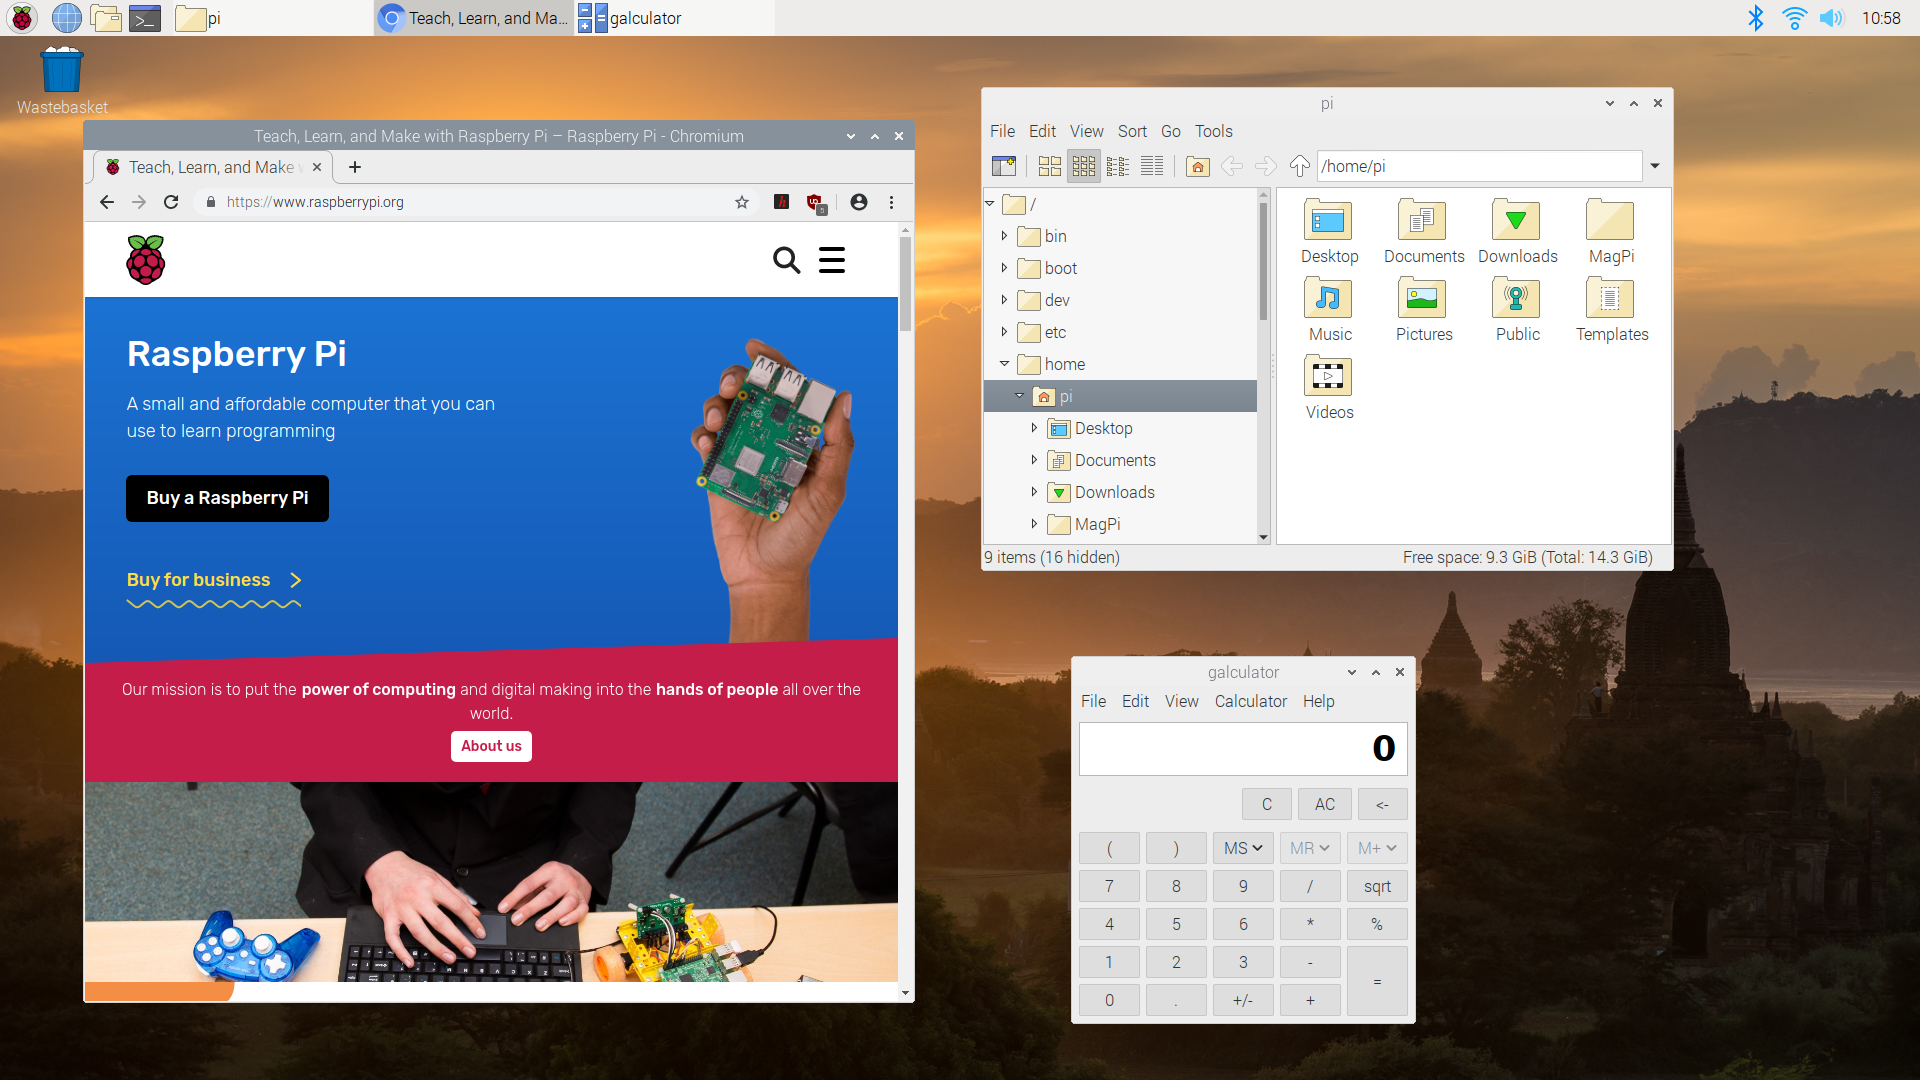
\includegraphics[width=15cm]{figures/chap3/interface_rpi_buster.png}
         \caption{affichage de bureau du raspberry buster}
\end{figure} 
 



 \subsection{les outils nécessaire au déploiement :}
 
Liste des librairies nécessaires au déploiement de modèle yolov5 sur Raspberry Pi:\\
  \begin{wrapfigure}{l}{0cm} 
{
\includegraphics[width=0.25\textwidth]{figures/chap3/cmake-logo.png}} \end{wrapfigure}permet de vérifier les pré requis nécessaires à la construction, de déterminer les dépendances entre les différents composants d'un projet, afin de planifier une construction ordonnée et adaptée à la plate-forme.
\newline
\vspace{10pt}
\begin{wrapfigure}{l}{1cm}{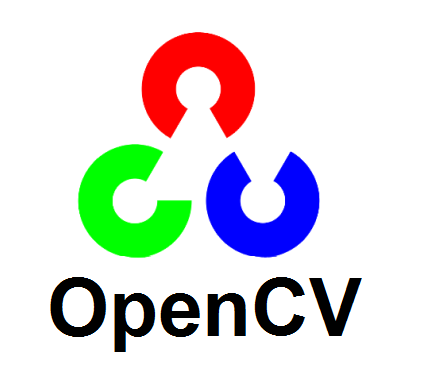
\includegraphics[width=0.25\textwidth]{figures/chap3/OpenCV_Logo.png}}\end{wrapfigure}La gestion du flux vidéo est géré par la célèbre libraire opencv.
\newline

\includegraphics[width=0.20\textwidth]{figures/chap3/pytorch.png}: est construit sur la base de la bibliothèque python et torch qui prend en charge les calculs de tenseurs sur les unités de traitement graphique. D'où  un tenseur est une unité fondamentale de données. Il peut s'agir d'un nombre, d'un vecteur, d'une matrice ou de tout tableau à n dimensions. Il est similaire aux tableaux Numpy. 
\newline

\includegraphics[width=0.20\textwidth]{figures/chap3/numpy.png} :Permet de créer directement un tableau depuis un fichier, de sauvegarder un tableau dans un fichier, et manipuler des vecteurs, matrices et polynômes.
\newline

\includegraphics[width=0.20\textwidth]{figures/chap3/pandas.png}:propose en particulier des structures de données et des opérations de manipulation de tableaux numériques et de séries temporelles.
\newline

\includegraphics[width=0.20\textwidth]{figures/chap3/scipy.png}:Projet qui consiste à unifier un ensemble de bibliothèques Python à usage scientifique.
\newline
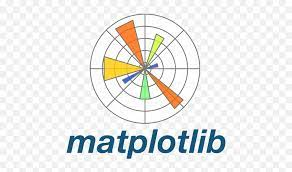
\includegraphics[width=0.20\textwidth]{figures/chap3/matplotlib.jpg} :destinée à tracer et visualiser des données sous formes de graphiques .
\newline

\includegraphics[width=0.20\textwidth]{figures/chap3/seaborn.png}:est une bibliothèque permettant de créer des graphiques statistiques en Python. Elle est basée sur Matplotlib, et s'intègre avec les structures Pandas.Elle permet d'explorer et de comprendre rapidement les données.\\
\section{Conclusion:}

 Tout au long de ce chapitre nous avons présenté 